\documentclass[tikz]{standalone}
\usetikzlibrary{spy,shapes,shadows,calc,pgfplots.groupplots}
\usepackage{amsmath}
\usepackage{physics} 
\usepackage{pgfplots}
\pgfplotsset{compat=1.3}
\usepackage{amsmath}
\DeclareFontFamily{OT1}{pzc}{}
\DeclareFontShape{OT1}{pzc}{m}{it}{<-> s * [1.10] pzcmi7t}{}
\DeclareMathAlphabet{\mathpzc}{OT1}{pzc}{m}{it}
\newcommand{\ddtn}{\operatorname{dtn}}

\pgfplotsset{
  legend style = {font=\small}
}

\begin{document}
\begin{tikzpicture}[scale = 0.8]



\begin{scope}[ ]
\node (diffB) at (0,2.5) {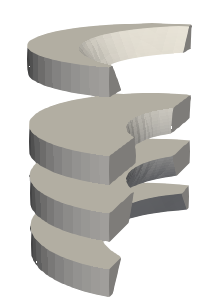
\includegraphics[scale =.35]{../plots/B-alpha-half.png}};
\draw[] (0,-0.175)   node[draw, fill=white, minimum size=0.5mm]{ $\kappa = 1/2 $ };
\end{scope}


\begin{scope}[xshift=2.5cm ]
\begin{groupplot}[
    group style={
        %group name=dtn,
        group size=1 by 1,
        %xticklabels at=edge bottom,
        horizontal sep=25pt,
        vertical sep=40pt,
   },
   %name = dtnplot,
   height = 6.5cm,
   width = 8.5cm,
   every axis plot/.append style={thick},
   %axis y line*=left,
   legend pos = south east,
   %ymin = 2e-6,
   %xmin = 0,
   %xmax = 11000,
   %ymin = -20,
   %ymax = 20,
   %restrict y to domain=-1e2:1e2,
   %label style={at={(axis description cs:0.5,-0.08)},anchor=north},
   %every x tick scale label/.style={at={(xticklabel cs:0.925)},anchor=south west},
   %x label style={at={(axis description cs:0.975,0.085)},anchor=east},
   %xlabel= { $\lambda$},
   ]
    
    \nextgroupplot[ 
    ymode=log,
    xmode=log,
    %xmin=0,xmax=1.6e4,
    %xtick={25, 125, 250, 500, 800, 1000},
    %axis x line*=middle,
    %axis y line=middle, 
    ymin = 6e-4,
    ymax = 6.0e-1,
    %width=9cm,
    %restrict y to domain=-4e2:4e2,
    %xtick={0,2e3,4e3,6e3,8e3,10e3,12e3,14e3},
    xlabel= { $ \sim h$},
    %legend pos = south west,
    legend style = { column sep = 10pt, legend columns = 5, legend to name = grouplegend, at={(0.5,-0.25)},anchor=north },
    x label style={at={(axis description cs:0.35,+0.06)},anchor=east},
	%title = {  $\norm{ u - \mathcal{L}_{\Delta t} \underline{u}_1 }_{L^2(Q)}$ },
	title = {    },
	]

    \addplot[red,very thick,mark=*,mark options={scale=0.75} ] 
   	table[x=deltat,y=L2-err-B] {../data/Cylinder--q1-qstar1-k1-kstar1-msol2.dat}; \addlegendentry{$ \kappa = 1$ }%
    \addplot[blue,very thick,mark=triangle*, mark options={scale=0.75}]  
	table[x=deltat,y=L2-err-B] {../data/Cylinder--q1-qstar1-k1-kstar1-msol2alpha-3quarter.dat};  \addlegendentry{$ \kappa = 3/4 $ }%
    \addplot[green!70!black,very thick,mark=diamond*, mark options={scale=0.75} ]  
	table[x=deltat,y=L2-err-B] {../data/Cylinder--q1-qstar1-k1-kstar1-msol2alpha-half.dat}; \addlegendentry{$ \kappa = 1/2 $ }%

    \addplot[magenta,very thick,mark=x, mark options={scale=0.75} ]  
	table[x=deltat,y=Qall] {../data/Cylinder--q1-qstar1-k1-kstar1-msol2alpha-quarter.dat}; \addlegendentry{$ Q $ }%

    \addplot[orange,very thick,mark=square*, mark options={scale=0.75} ]  
	table[x=deltat,y=L2-err-B] {../data/Cylinder--q1-qstar1-k1-kstar1-msol2alpha-quarter.dat}; \addlegendentry{$ \kappa = 1/4 $ }%

    \addplot[lightgray,dotted,ultra thick] 
	table[mark=none,x=deltat,y expr ={1.25*\thisrowno{0}*\thisrowno{0} }] {../data/Cylinder--q1-qstar1-k1-kstar1-msol2.dat}; \addlegendentry{$ \mathcal{O}(h^2) $ }%

    \addplot[lightgray,dashed,ultra thick] 
	table[mark=none,x=deltat,y expr ={.75*\thisrowno{0}*\thisrowno{0}^0.5 }] {../data/Cylinder--q1-qstar1-k1-kstar1-msol2.dat}; \addlegendentry{$ \mathcal{O}(h^{1.5}) $ }%

    \addplot[lightgray,dashdotted,ultra thick] 
	table[mark=none,x=deltat,y expr ={.25*\thisrowno{0}^0.8 }] {../data/Cylinder--q1-qstar1-k1-kstar1-msol2.dat}; \addlegendentry{$ \mathcal{O}(h^{0.8}) $ }%

    \addplot[lightgray,thick] 
	table[mark=none,x=deltat,y expr ={  0.45/ abs(ln(  (\thisrowno{0} ) ) )  } ] {../data/Cylinder--q1-qstar1-k1-kstar1-msol2.dat}; \addlegendentry{$ \mathcal{O}( \vert \log(h) \vert^{-1}  ) $ }%

     \node (diffC) at (axis cs:0.275,7e-3) {
\includegraphics[scale =.25]{../plots/B-alpha-one.png}};
     \draw[] (axis cs:0.29,1e-3)   node[draw, fill=white, minimum size=0.3mm]{ $\kappa = 1 $ };

    \end{groupplot}
    \node at ($(group c1r1) + (0.0cm,-3.75cm)$) {\ref{grouplegend}}; 
\end{scope}


\begin{scope}[xshift=12cm ]
\node (diffB) at (0,2.5) {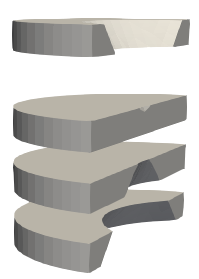
\includegraphics[scale =.35]{../plots/B-alpha-quarter.png}};
	\draw[] (0,-0.175)   node[draw, fill=white, minimum size=0.5mm]{ $\kappa = 1/4 $  };
\end{scope}

\end{tikzpicture}
\end{document}





